\documentclass{article}

\usepackage{float}
\usepackage{xcolor}
\usepackage{parskip}
\usepackage{eulervm}
\usepackage{graphicx}
\usepackage{setspace}
\usepackage{geometry}
\usepackage{microtype}
\usepackage[T1]{fontenc}
\usepackage[utf8]{inputenc}
\usepackage{amsfonts, amsmath, amssymb}

\setstretch{1.50}
\geometry{paper=letterpaper, layout=letterpaper, margin=1in}

\begin{document}

\begin{titlepage}
    \begin{center}
        \vspace*{2cm}
        {\Huge \textbf{ ME 4638: Computational Mechanics Lab}} \\
        \vspace{1cm}
        {\Large \textbf{Assignment IV \& V}} \\

        \vfill

        \textit{\large Submitted by:} \\
        \vspace{0.3cm}
        \textbf{Abdullah al Azmi, 220011230} \\
        % \textbf{Std. ID: 220011230} \\

        \vfill

        \textit{\large Submitted to:} \\
        \vspace{0.3cm}
        \textbf{\Large Sefat Mahmud Siddique} \\
        \textbf{Junior Lecturer, Department of Mechanical and Production Engineering} \\

        \vfill

        \textbf{Date of Submission: \today}
        \vspace*{1cm}
    \end{center}
\end{titlepage}

\newpage

\section*{Experiment 4}

\subsection*{Problem I}

\subsubsection*{No. of node: 20}

\begin{figure}[H]
    \centering
    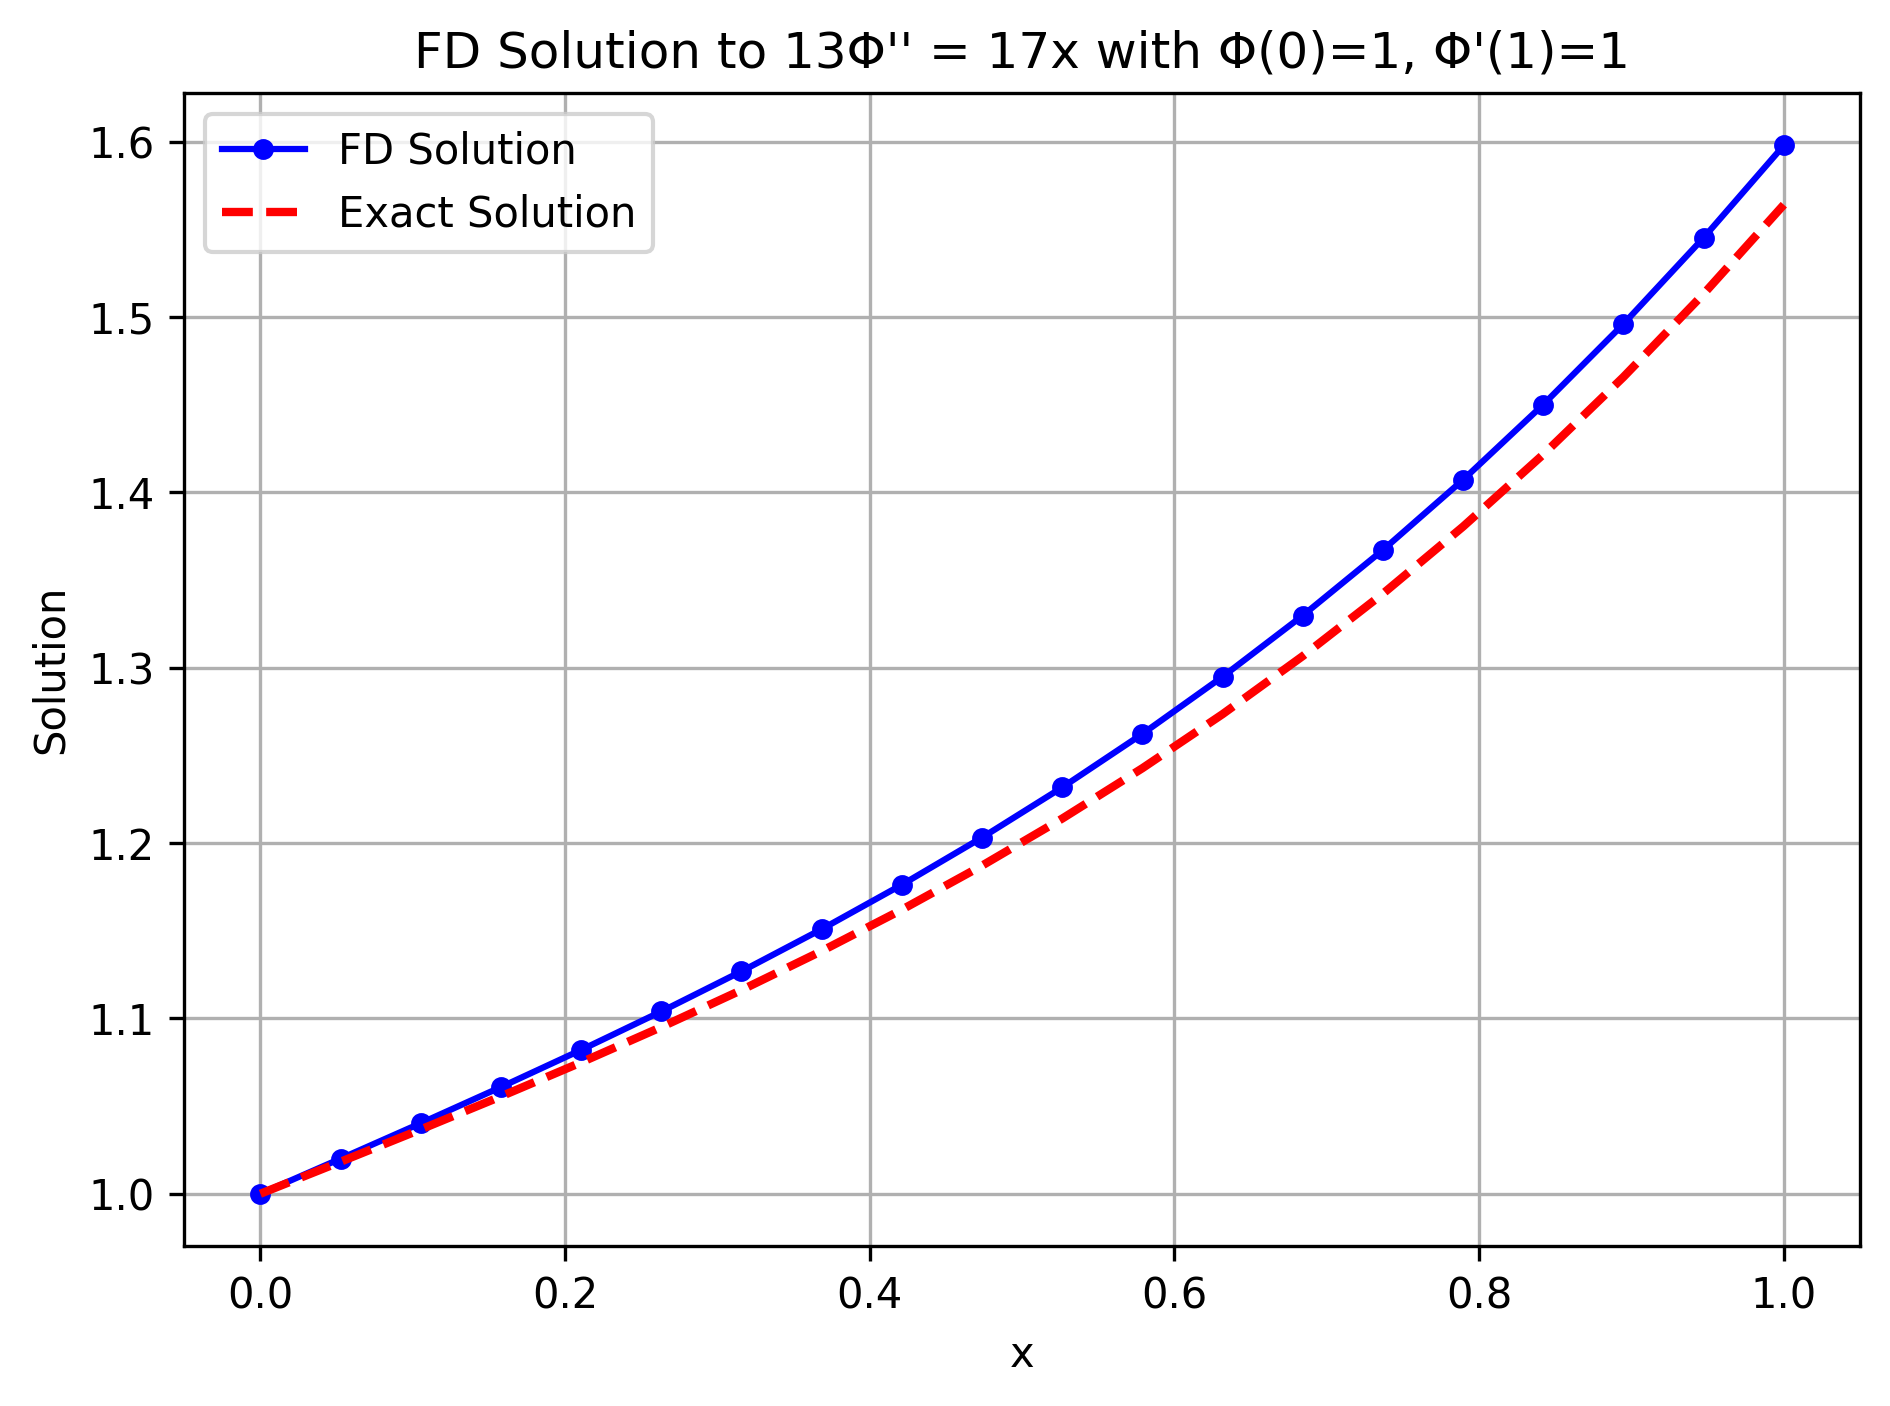
\includegraphics[width=0.75\textwidth]{images/node_20.png}
\end{figure}

\subsubsection*{No. of node: 100}

\begin{figure}[H]
    \centering
    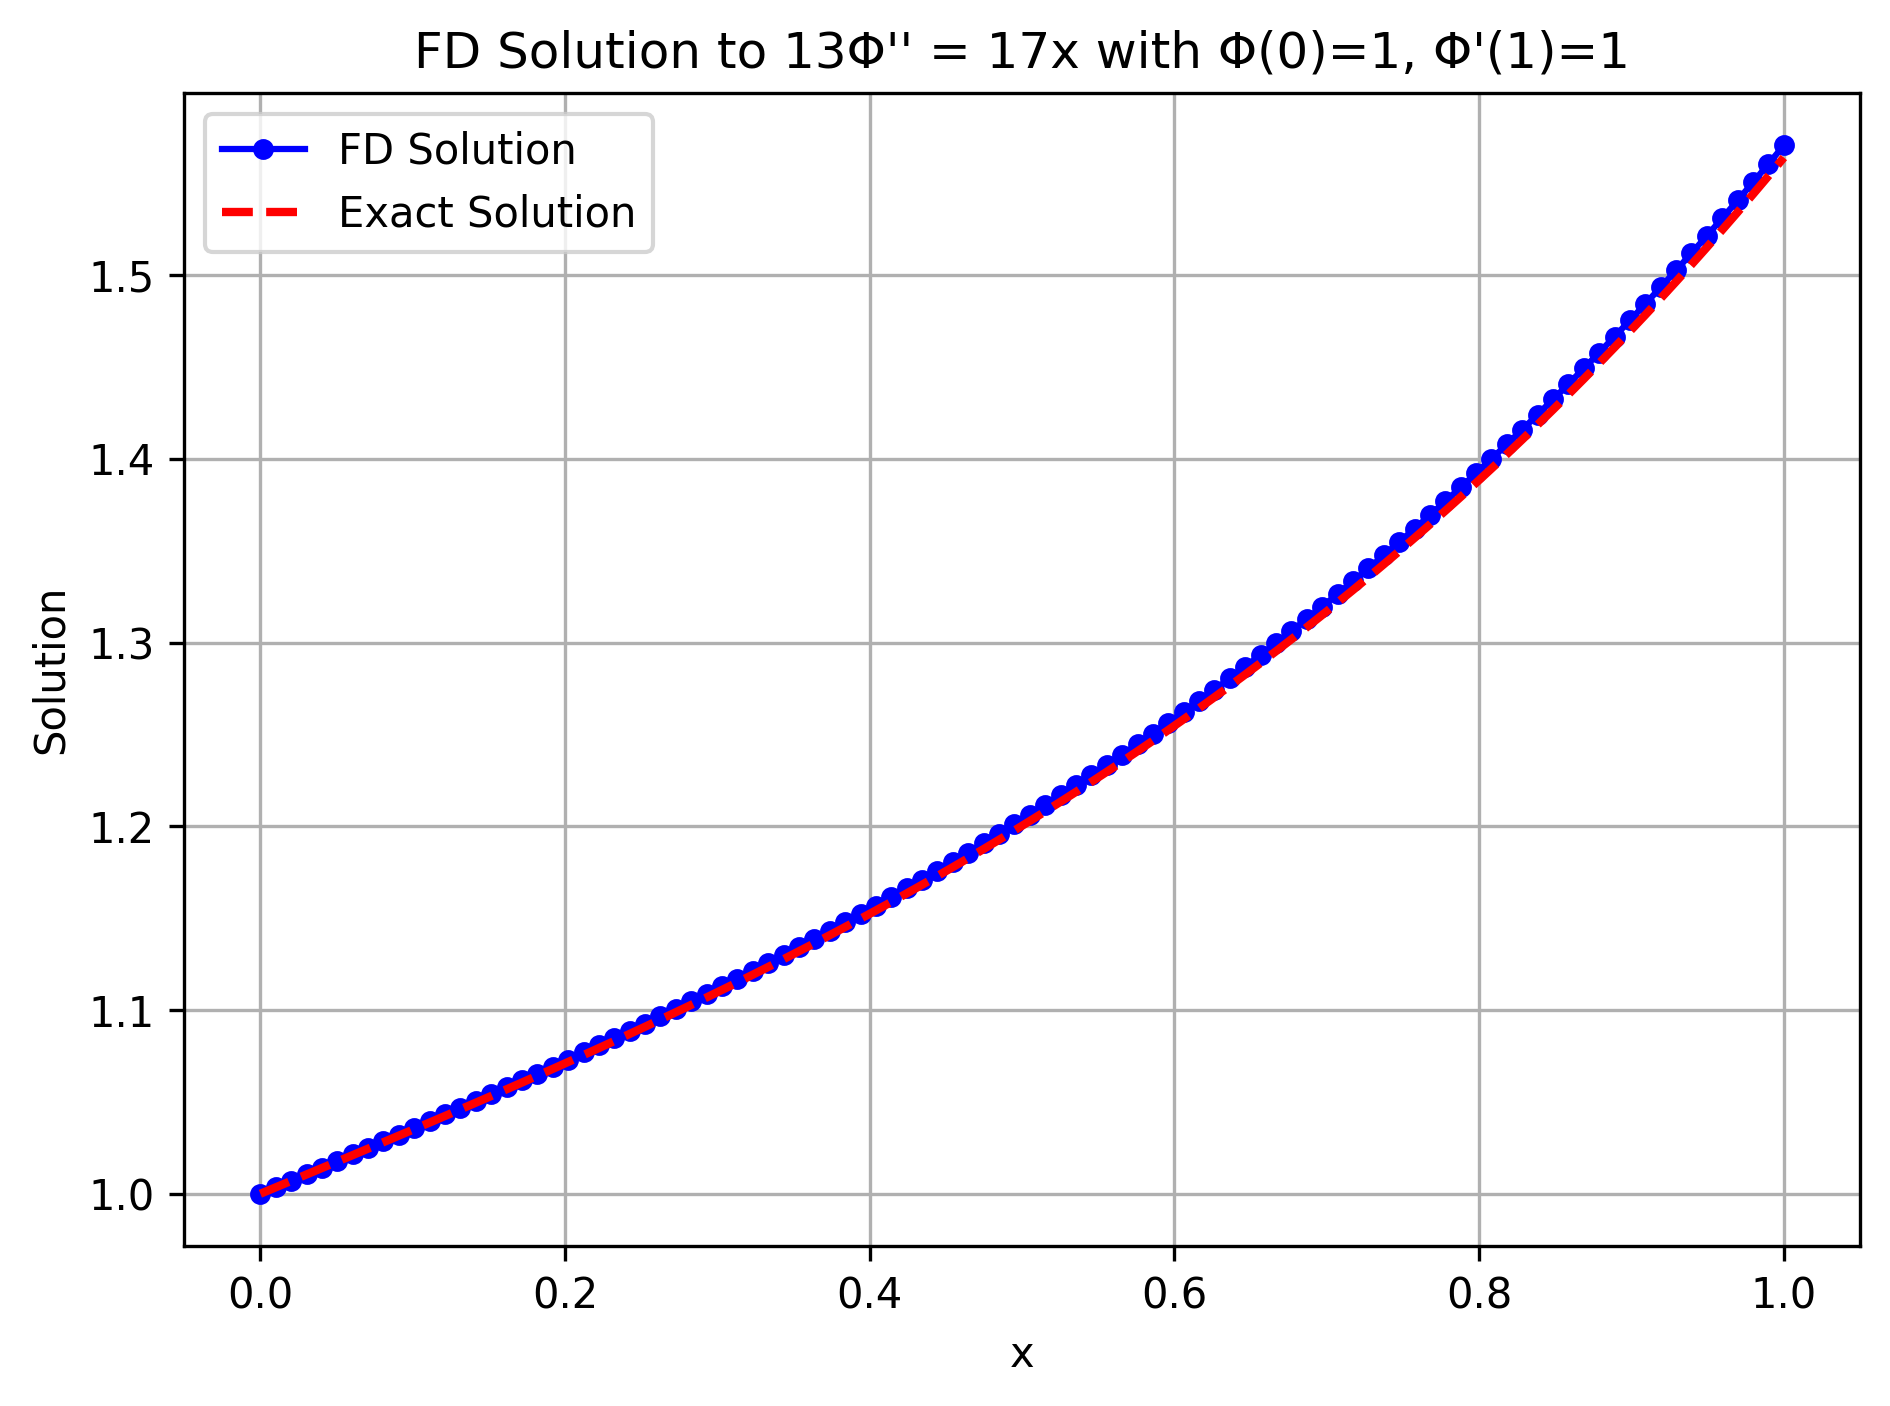
\includegraphics[width=0.75\textwidth]{images/node_100.png}
\end{figure}



\section*{Problem II}

As the number of node increase, the numerical solvers becomes able to capture the tiny or small relationship in the equations like the one in graph or in calculus where the smaller the dx, the refiner or exact the solutions.

\section*{Problem III}

In neumann boundary condition, we know the exact value and that matches with our results in case of second one, when the number of node was 100. But, for dirichlet boundary condition, as we do not know that exact value, rather we have the differentiation form. This matches when our node was 20, and we observed the differentiation does not become zero.

Obviously, the neumann boundary condition provides better accuracy as we know the exact value.

\section*{Problem IV}

If the boundary conditions were dirichlet boundary condition, then the solution would never converged.

\newpage

\section*{Experiment 5}

\subsection*{Problem I}

\begin{figure}[H]
    \centering
    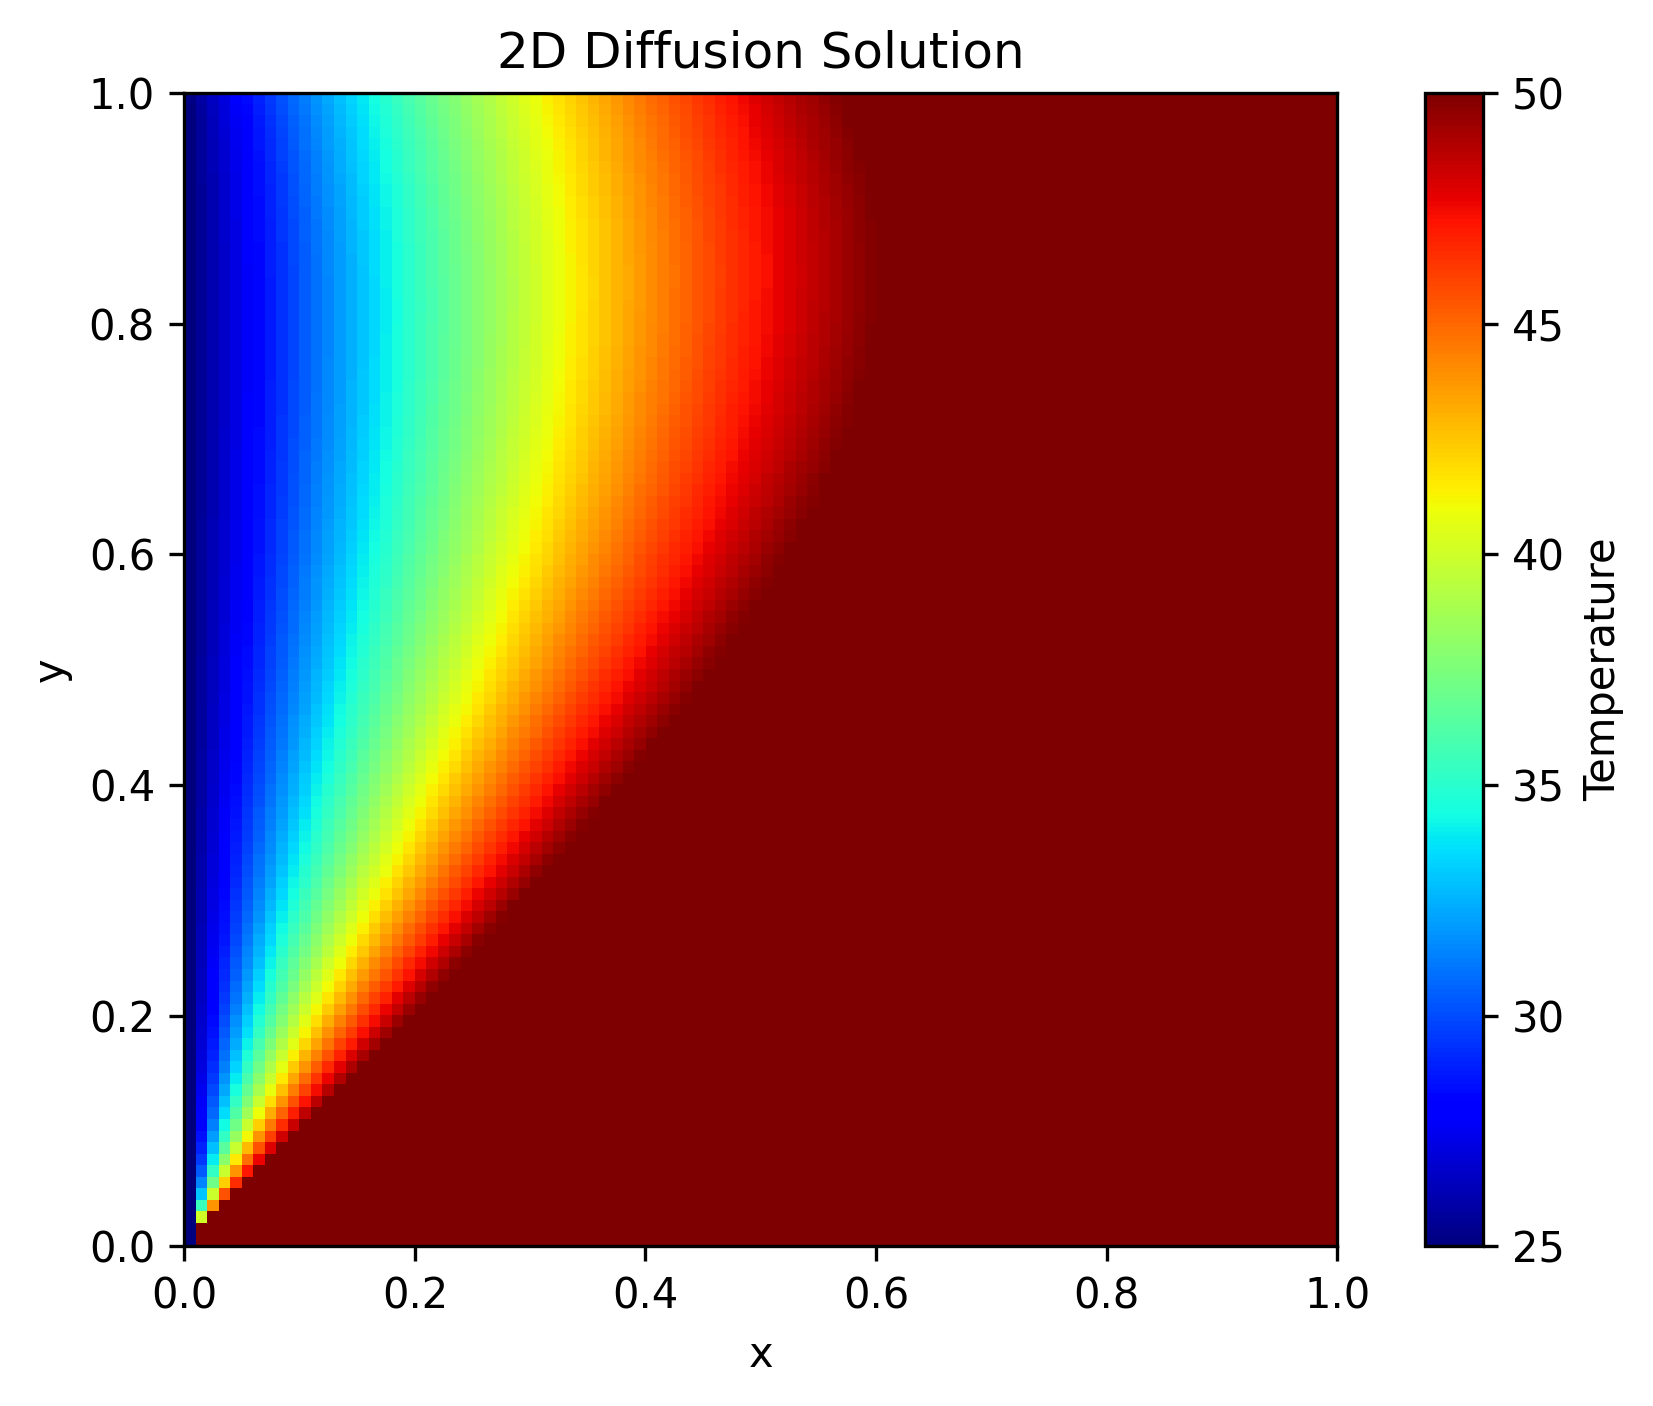
\includegraphics[width=0.65\textwidth]{images/basic_figure.png}
\end{figure}

\subsection*{Problem II}

\begin{figure}[H]
    \centering
    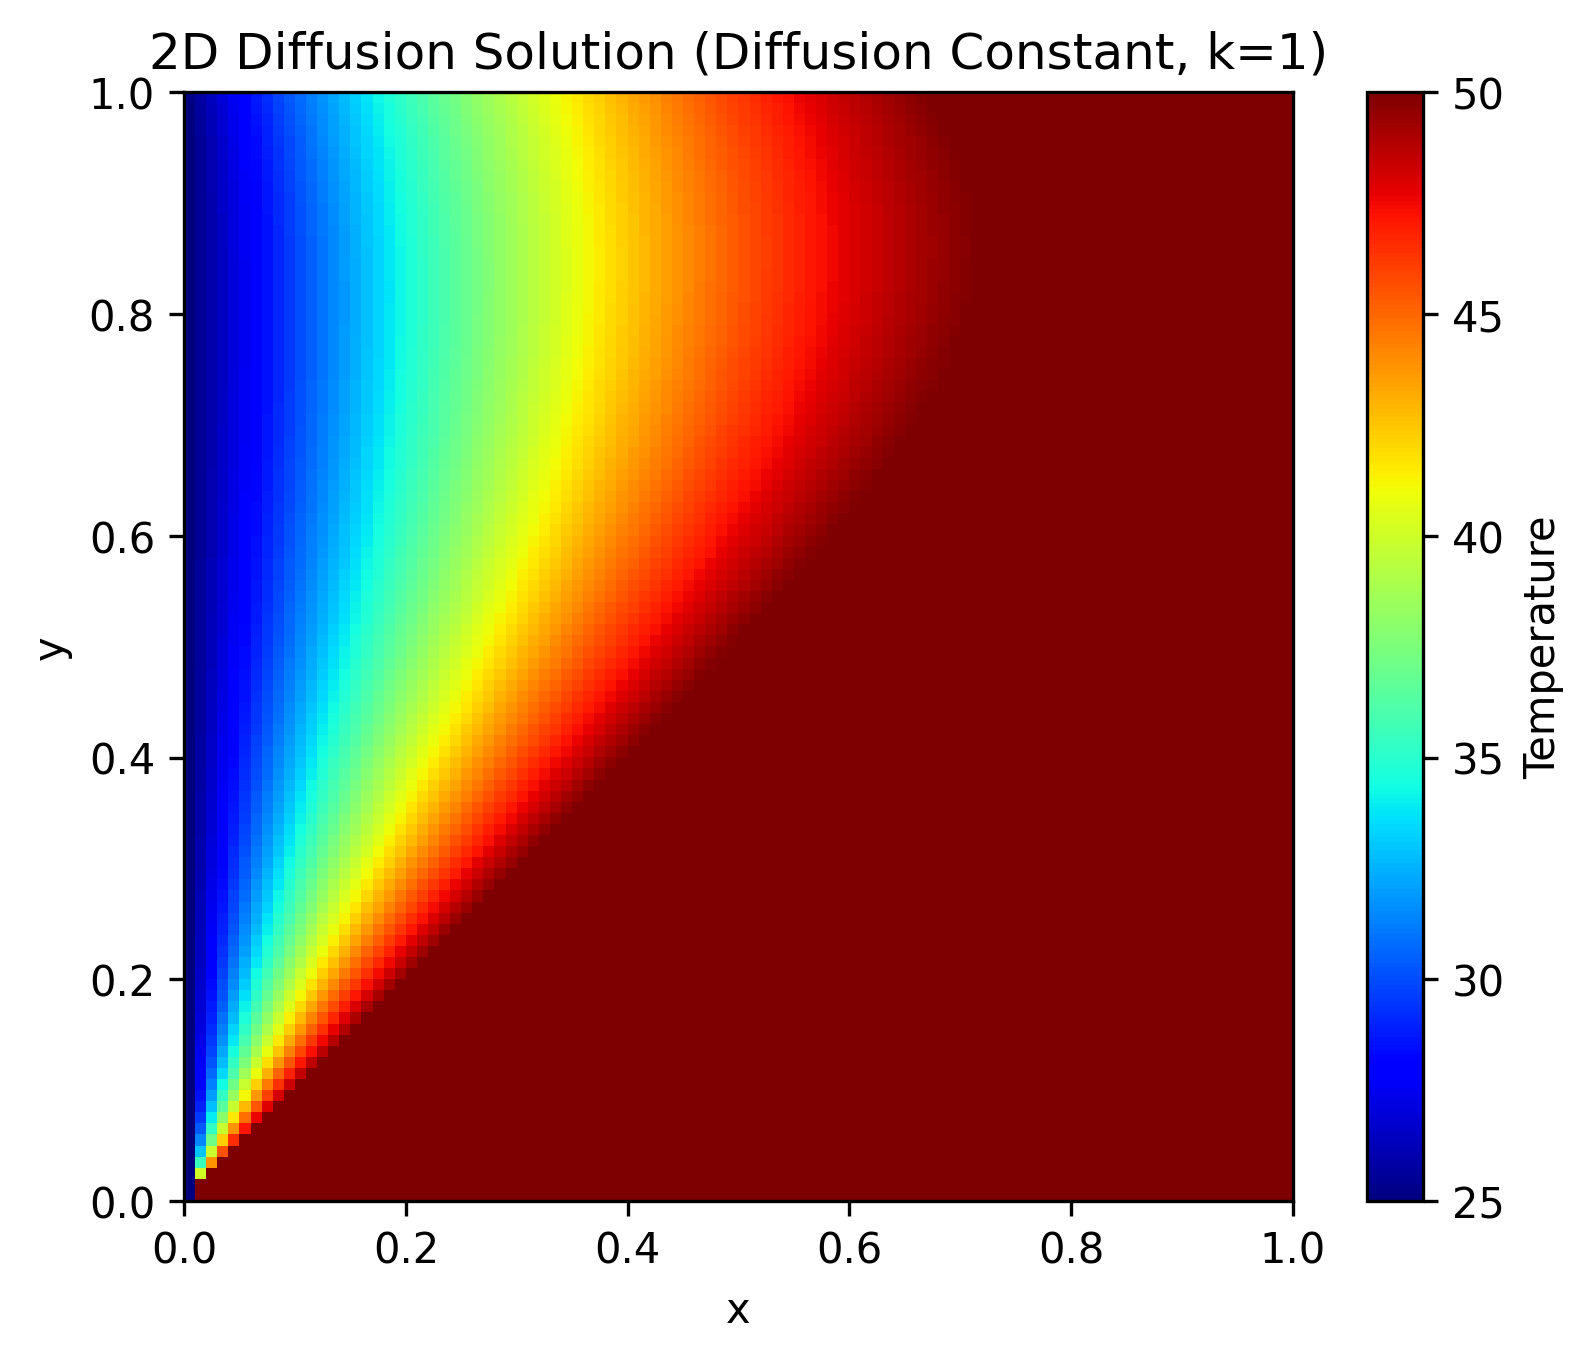
\includegraphics[width=0.65\textwidth]{images/diffusion_const_1.png}
\end{figure}

\begin{figure}[H]
    \centering
    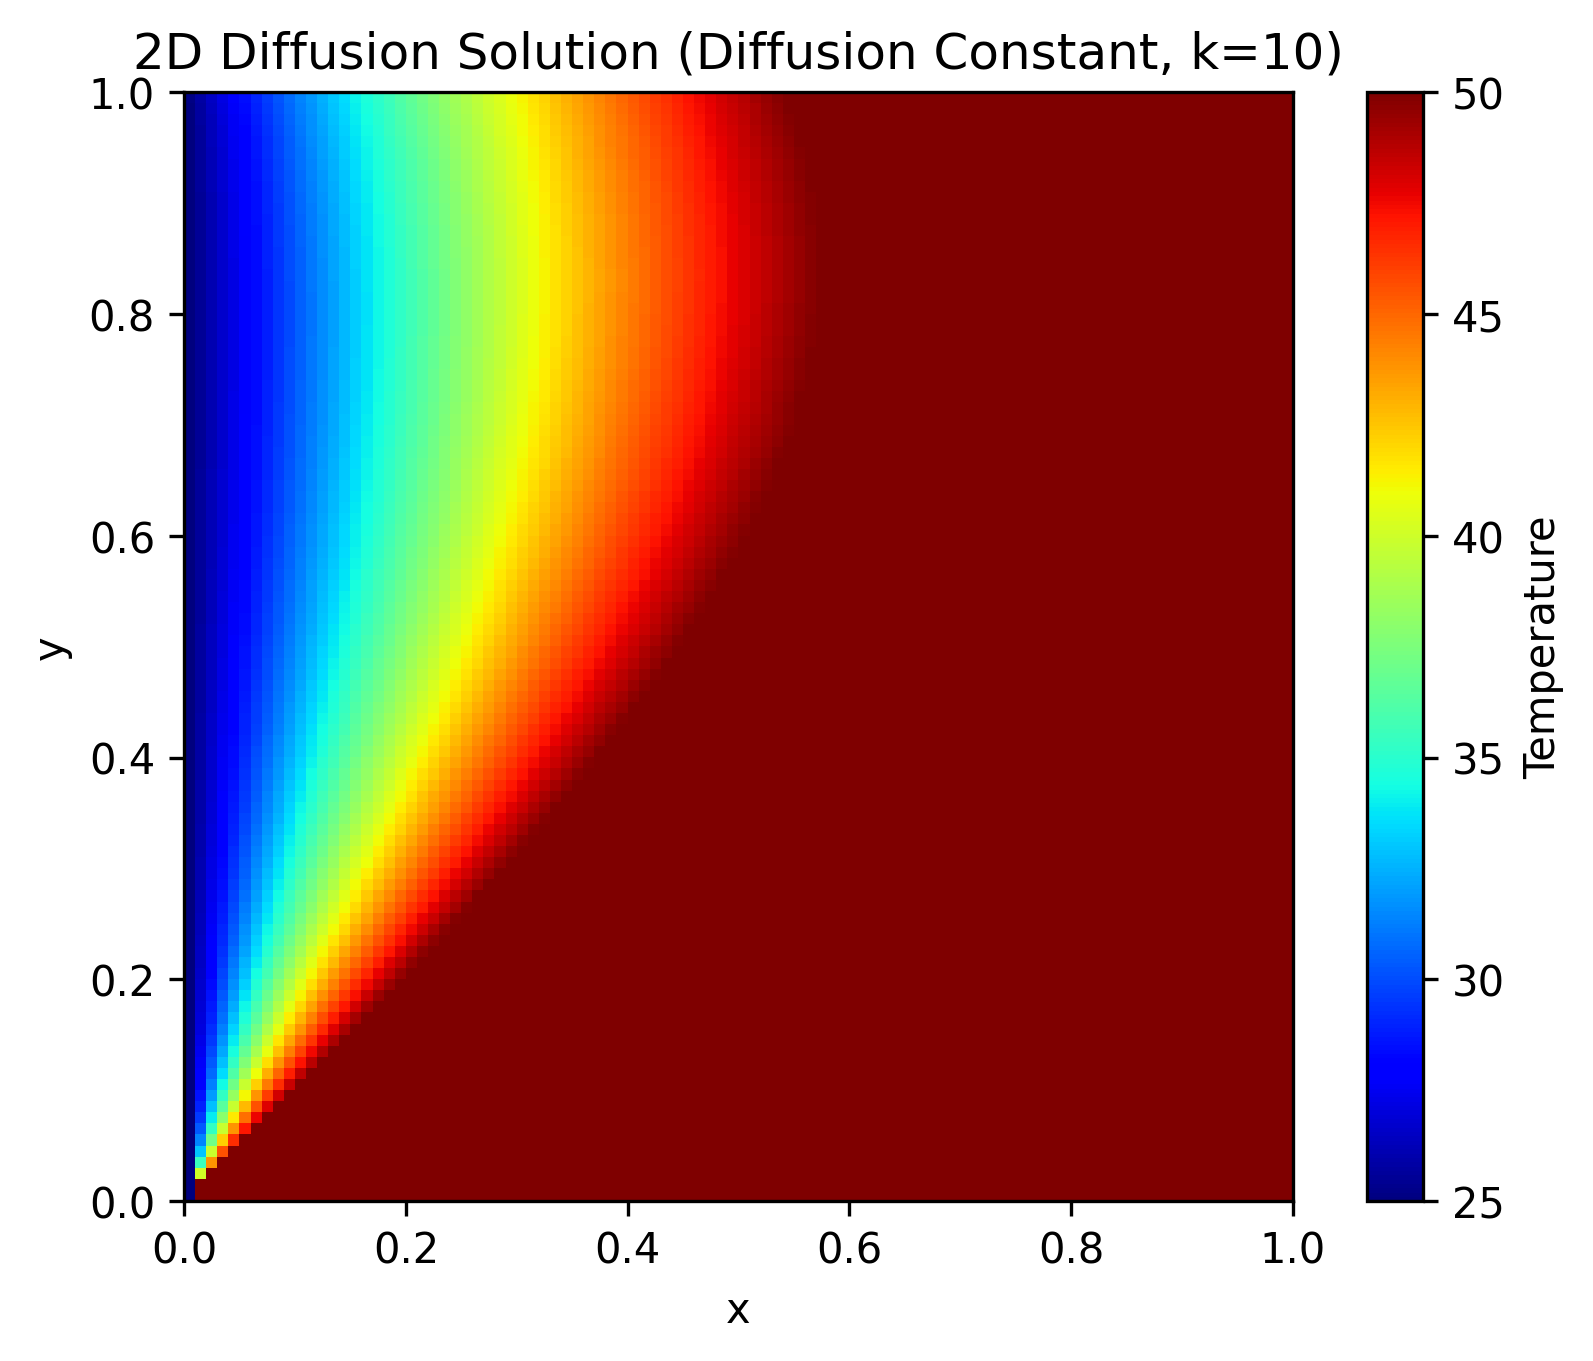
\includegraphics[width=0.65\textwidth]{images/diffusion_const_10.png}
\end{figure}

\begin{figure}[H]
    \centering
    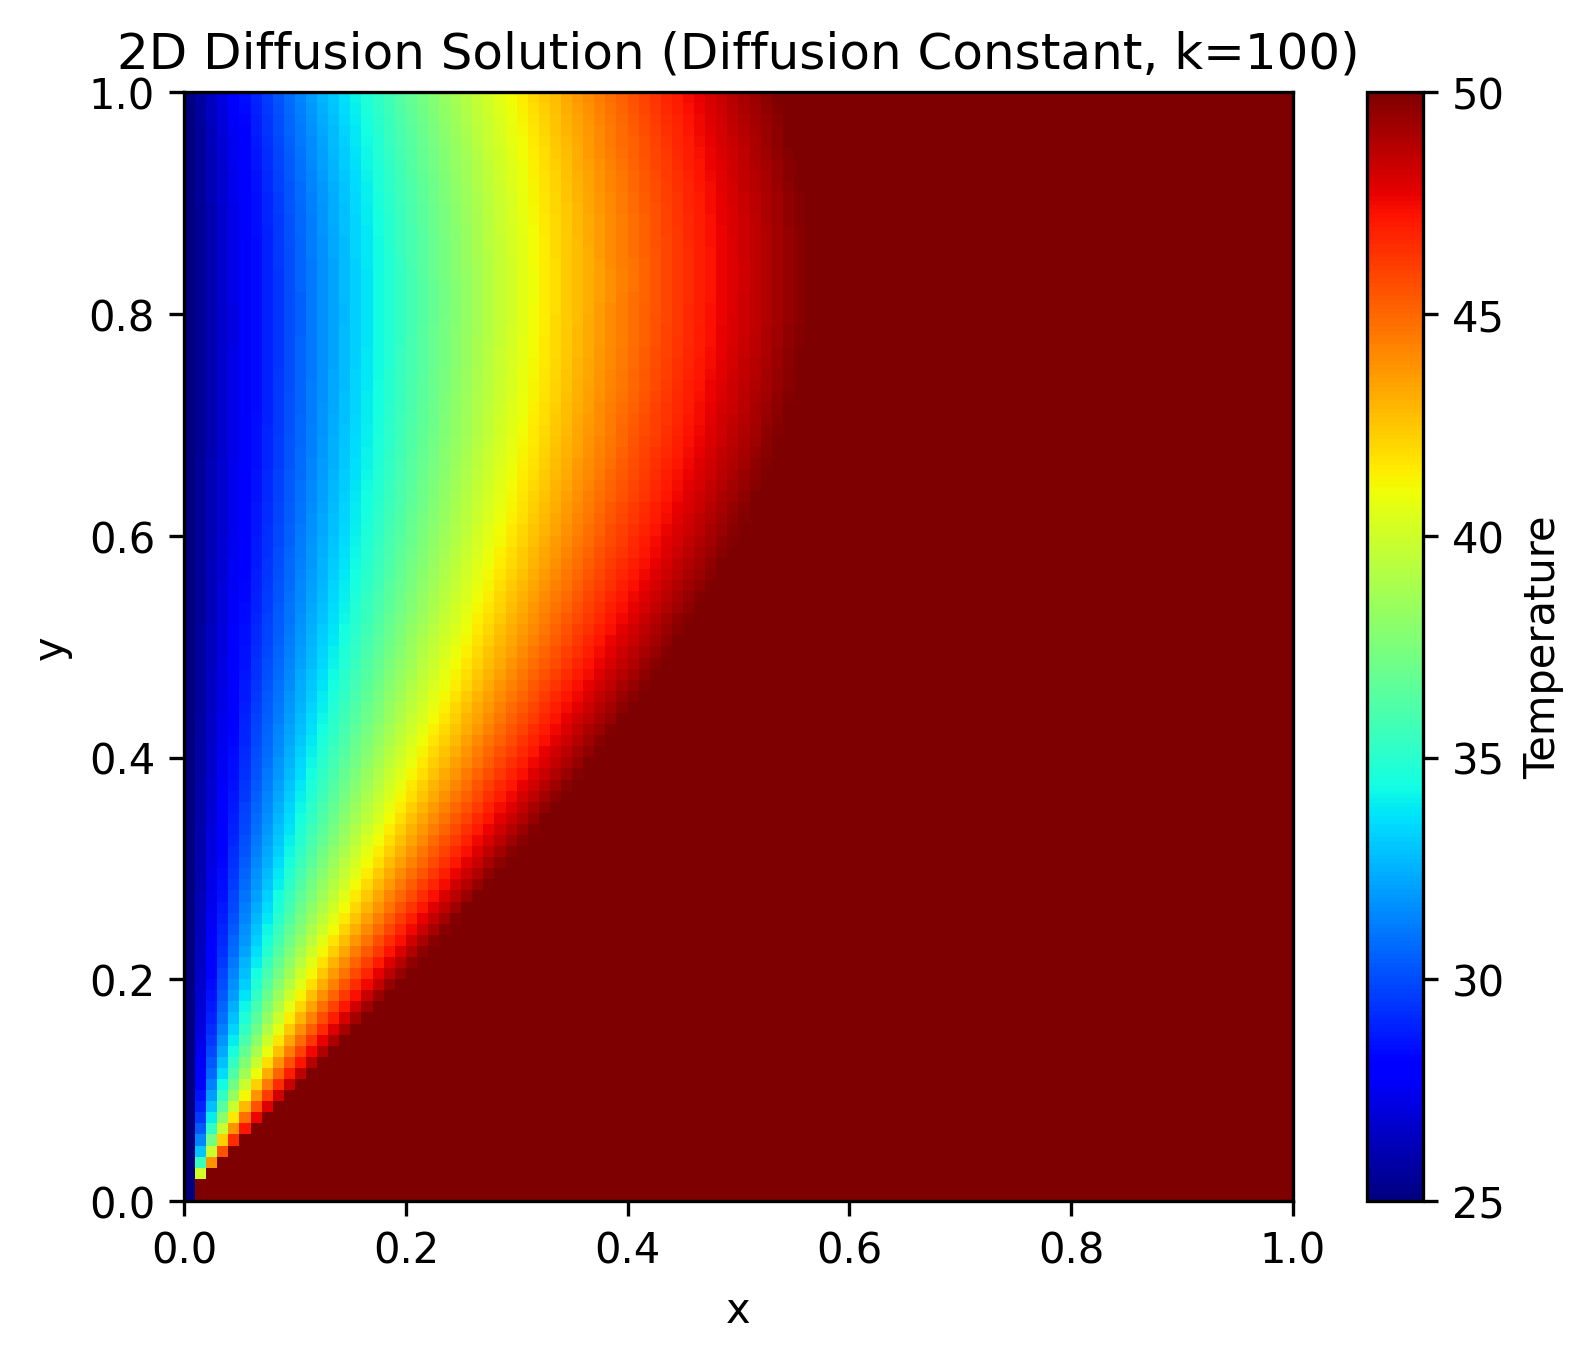
\includegraphics[width=0.65\textwidth]{images/diffusion_const_100.png}
\end{figure}

\end{document}